\documentclass{beamer}

\usepackage{graphicx, amsmath, amsthm, amssymb, tikz, listings}

\lstset{language=C, frame=single}

\definecolor{UDBlue}{RGB}{0,83,159}
\definecolor{UDGold}{RGB}{255,210,0}

\usetheme{Madrid}
\usecolortheme[RGB={0,83,159}]{structure}
\setbeamertemplate{blocks}[rounded][shadow=true]
\useoutertheme{split}
\beamertemplatenavigationsymbolsempty

\author{Ryan McKenna, Matthew Paul, James Kerrigan \\
Niko Gerassimakis, Neil Duffy }
\title{Team 6: LU Factorization}
\subtitle{Optimizations targeting towards multicore processors}
\date{\today}

\logo{
	
\includegraphics[height=1cm, keepaspectratio]{delaware_logo.png}
}

\begin{document}

\frame{\maketitle}

\begin{frame}

\frametitle{Linear Algebra}

\begin{itemize}
\item The quintessential problem in linear algebra is solving a linear system of equations

$$
\begin{bmatrix}
	a_{11} &  a_{12} &  a_{13}  \\
	a_{21}  &  a_{22} &  a_{23}  \\
	a_{31}  &  a_{32}  &  a_{33}
\end{bmatrix}
\begin{bmatrix}
x_1\\x_2\\x_3
\end{bmatrix}
=
\begin{bmatrix}
b_1\\b_2\\b_3
\end{bmatrix}
$$

\item We want to find values of $ x_1, x_2, $ and $ x_3 $ such that 

\begin{enumerate}
\item $ a_{11} x_1 + a_{12} x_2 + a_{13} x_3 = b_1 $
\item $ a_{21} x_1 + a_{22} x_2 + a_{23} x_3 = b_2 $
\item $ a_{31} x_1 + a_{32} x_2 + a_{33} x_3 = b_3 $
\end{enumerate}

\end{itemize}

\end{frame}


\begin{frame}
\frametitle{Impact}

\begin{itemize}
\item Linear algebra comes up in a lot of professions:
\begin{itemize}
\setlength\itemsep{0.25em}
\item Physics
\item Partial differential equations
\item Graph theory
\item Statistics / Curve Fitting
\item Sports Ranking
\end{itemize}

\end{itemize}
	
\end{frame}


\begin{frame}
\frametitle{Solving Linear Systems}

\begin{itemize}
\item If $A$ is an $ n $ x $ n $ matrix, solving a system of the form $ A x = b $ takes $ O(n^3) $ time.

\item If $ A$ is a triangular matrix, then solving the system takes $ O(n^2) $ time
\end{itemize}
\end{frame}

\begin{frame}
\frametitle{LU Factorization Background}

\begin{itemize}
\item LU Factorization works by decomposing a square matrix $A$ into a lower triangular matrix, $L$, and an upper triangular matrix, $U$:

$$ A = L U $$

$$ 
\begin{bmatrix}
	a_{11} &  a_{12} &  a_{13}  \\
	a_{21}  &  a_{22} &  a_{23}  \\
	a_{31}  &  a_{32}  &  a_{33}
\end{bmatrix}
=
\begin{bmatrix}
	l_{11} &  0 &  0  \\
	l_{21}  &  l_{22} &  0  \\
	l_{31}  &  l_{32}  &  l_{33}
\end{bmatrix}
\begin{bmatrix}
	u_{11} &  u_{12} &  u_{13}  \\
	0  &  u_{22} &  u_{23}  \\
	0  &  0  &  u_{33}
\end{bmatrix}
$$

\item With $ L $ and $ U $, we can solve $ A x = L U x = b $ in $ O(n^2) $.  


\end{itemize}
\end{frame}

\begin{frame}
\frametitle{Algorithm Description / Access Pattern}

LU factorization is an $ O(n^3) $ algorithm:

\begin{center}
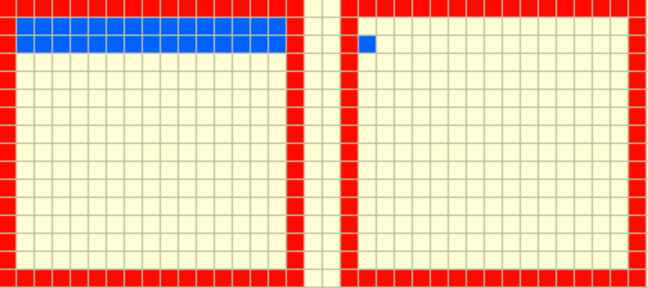
\includegraphics[scale=0.2]{figures/lu1a}\hspace{1em}
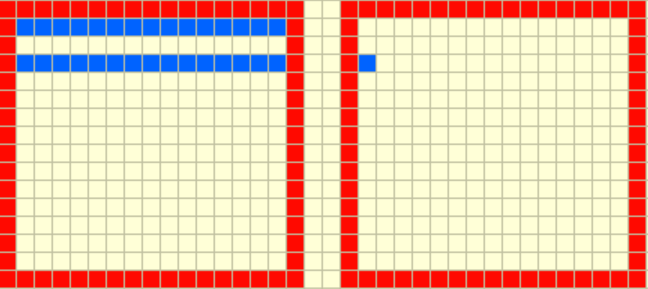
\includegraphics[scale=0.2]{figures/lu1b}
\hspace{1em}
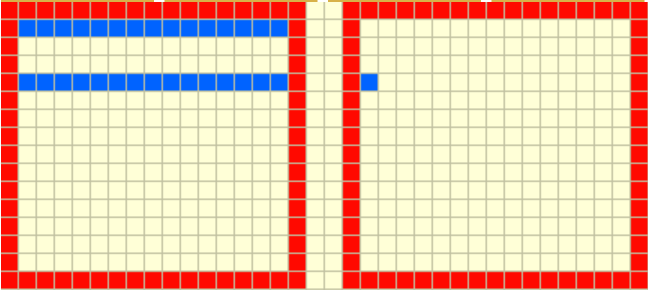
\includegraphics[scale=0.2]{figures/lu1c}
\hspace{1em}
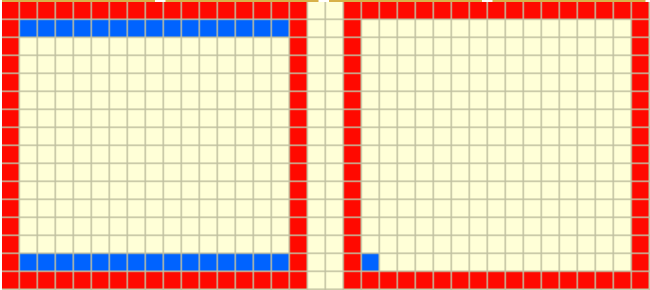
\includegraphics[scale=0.2]{figures/lu2} 


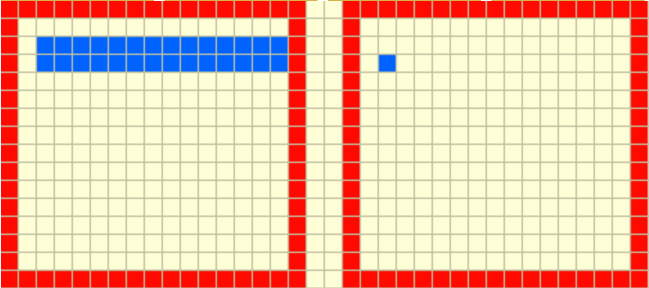
\includegraphics[scale=0.2]{figures/lu3}
\hspace{1em}
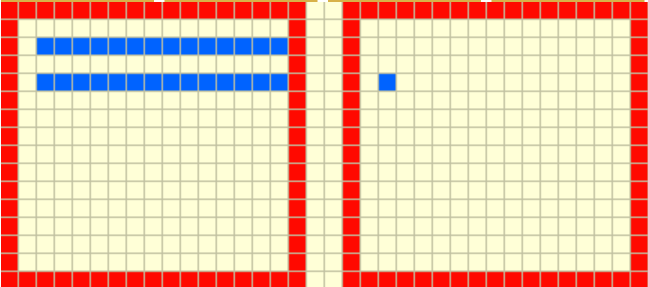
\includegraphics[scale=0.2]{figures/lu4}
\hspace{1em}
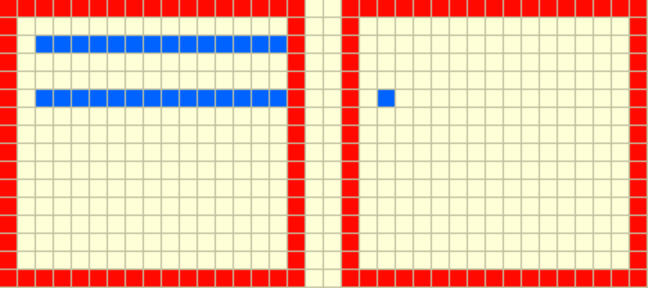
\includegraphics[scale=0.2]{figures/lu2b}
\hspace{1em}
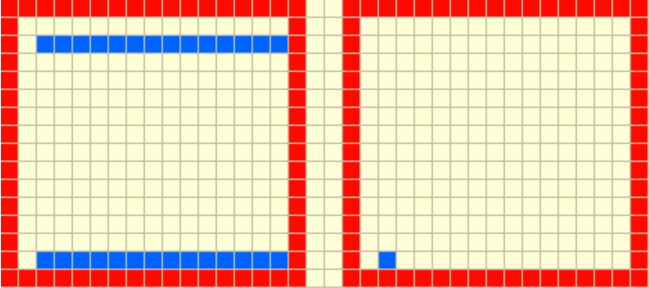
\includegraphics[scale=0.2]{figures/lu5}
$$\vdots$$
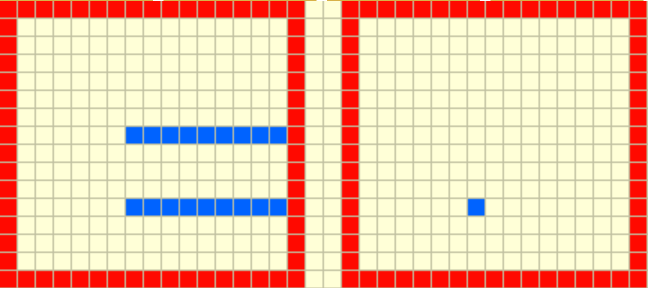
\includegraphics[scale=0.2]{figures/lu6}
$$\vdots$$
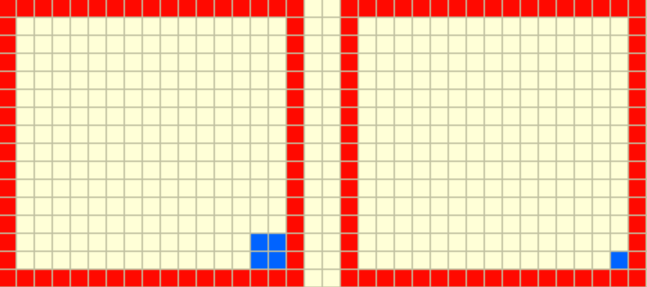
\includegraphics[scale=0.2]{figures/lu7}
\end{center}

\end{frame}


\begin{frame}[fragile]
\frametitle{Implementation}

\begin{lstlisting}
void lu(double **A, double **L, double **U, int n) {
    zero (L, n);
    copy (U, A, n);
    init (L, n);
    for(int j=0; j < n; j++) {
        for(int i=j+1; i < n; i++) {
            double m = U[i][j] / U[j][j];
            L[i][j] = m;
            for(int k=j; k < n; k++)
                U[i][k] -= m*U[j][k];
        }
    }
}
\end{lstlisting}

\end{frame}


\begin{frame}
\frametitle{Architecture}
\begin{itemize}

\item 


\end{itemize}
\end{frame}

\begin{frame}
\frametitle{Approach}
\begin{enumerate}
\item Generate random matrices up to 6400 x 6400.
\item Run and time 4 trials of the factorization algorithm for each matrix size.
\item Repeat for every optimization configuration.
\end{enumerate}
\end{frame}

\begin{frame}
\frametitle{Optimizations}

\begin{itemize}
\item -O1, -O2, -O3
\item loop unrolling
\item vectorization
\item native (architecture specific) optimizations
\item openMP
\end{itemize}

\end{frame}

\begin{frame}
\frametitle{Compiler}



\end{frame}

\begin{frame}[fragile]
\frametitle{Sequential Results}

\begin{tabular}{|c|c|c|c|c|c|c|c|}
\hline
& \multicolumn{7}{|c|}{Optimization / Time (s)} \\
\hline
n & None & -O1 & -O2 & Vector & -O3 & Unroll & Native\\
\hline
100	& 0.0028 & 0.0010 & 0.0008 & 0.0005 & 0.0005 & 0.0004 & 0.0003 \\
200	& 0.0101 & 0.0034 &	0.0026 & 0.0017 & 0.0018 & 0.0025 & 0.0014 \\
400	& 0.07902 & 0.0219 & 0.0189 & 0.0158 & 0.01561 & 0.0151 & 0.0124 \\
800	& 0.6222 & 0.1575 & 0.1070 & 0.0850 & 0.0821 & 0.0800 & 0.0662 \\
1600 & 4.9364 & 1.3342 & 0.9388 & 0.7737 & 0.7900 & 0.7465 & 0.6732 \\
3200&39.7114 & 11.7545 & 9.5557 & 8.4604 &	8.4156 & 8.1363 & 8.0514 \\
6400 & 316.3 & 94.23 & 78.12 &	69.35 & 68.70 & 66.54 & 66.76\\
\hline
\end{tabular}

\begin{itemize}
\setlength\itemsep{0.25em}
\item Going from no optimizations to -O1 gave nearly 400\% speedup.  
\item Vectorization yielded an 11\% speedup.
\item Loop unrolling gave a 3 \% speedup in the largest case.
\item Native optimizations yieled a 15 \% speedup in the best case (n = 1600).  
\end{itemize}

\end{frame}

\begin{frame}
\frametitle{Sequential Results}

\begin{center}
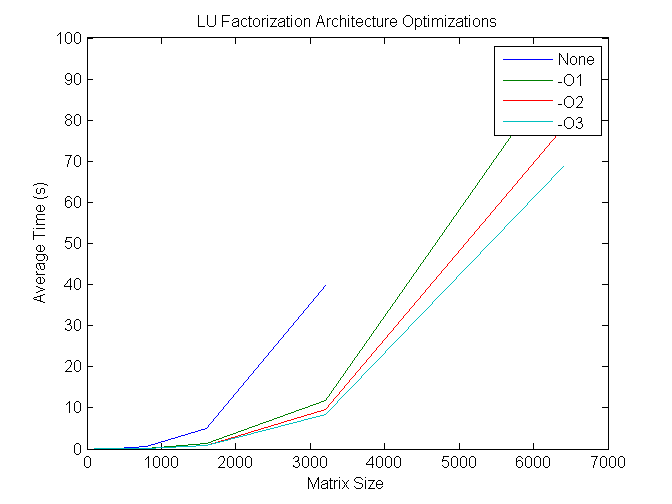
\includegraphics[scale=0.5]{figures/fig2}
\end{center}

\end{frame}

\begin{frame}
\frametitle{Sequential Results}

\begin{center}
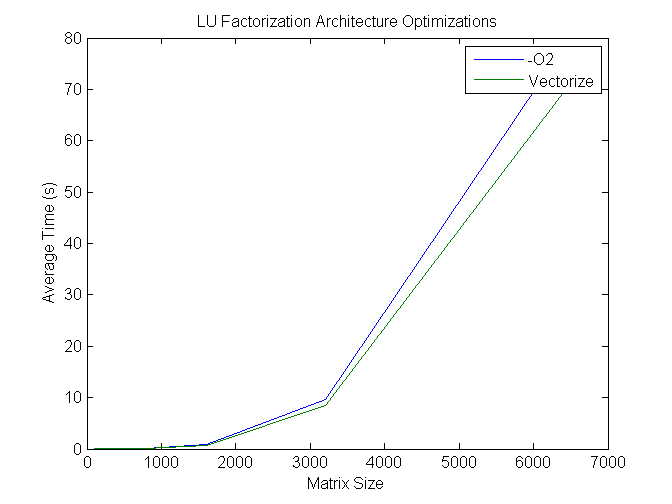
\includegraphics[scale=0.5]{figures/fig3}
\end{center}

\end{frame}

\begin{frame}
\frametitle{Sequential Results}

\begin{center}
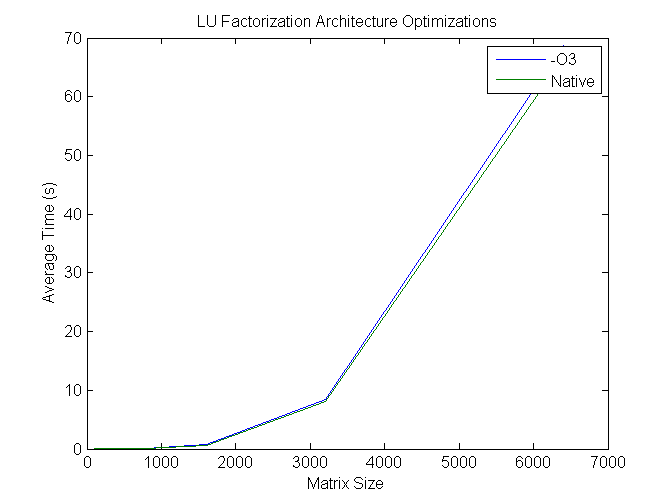
\includegraphics[scale=0.5]{figures/fig4}
\end{center}

\end{frame}

\begin{frame}[fragile]
\frametitle{Parallel Implementation}

\begin{lstlisting}
void lu(double **A, double **L, double **U, int n) {
    zero (L, n);
    copy (U, A, n);
    init (L, n);
    for(int j=0; j < n; j++) {
        #pragma omp parallel for schedule(static,8)  
        for(int i=j+1; i < n; i++) {
            double m = U[i][j] / U[j][j];
            L[i][j] = m;
            for(int k=j; k < n; k++)
                U[i][k] -= m*U[j][k];
        }
    }
}
\end{lstlisting}

\end{frame}

\begin{frame}[fragile]
\frametitle{Parallel Results}

\begin{center}
\begin{tabular}{|c|c|c|c|c|}
\hline
n & Native & 2 Threads & 4 Threads & 8 Threads\\
\hline
100	& 0.000338 & 	0.000337 & 0.001492	& 0.000409 \\
200	& 0.001417 & 	0.0014 & 0.000963 &	0.000725 \\
400	& 0.012435 & 0.006679 & 0.003321 & 0.002973 \\
800	& 0.066184 & 0.036134 & 0.02161 & 0.021725 \\
1600 & 0.6732 &	0.354768 & 0.221714 & 0.219362 \\
3200 & 8.05138 & 4.457911 & 3.46599 & 3.567894 \\
6400 & 66.760086 & 36.836628 & 28.870047 & 30.108377 \\
\hline
\end{tabular}
\end{center}

\begin{itemize}
\setlength\itemsep{0.25em}
\item From 1 core to 2 cores, we achieved a scalability of 1.81. 
\item Past 2 cores, we saw diminishing returns.  
\end{itemize}

\end{frame}

\begin{frame}
\frametitle{Parallel Results}

\begin{center}
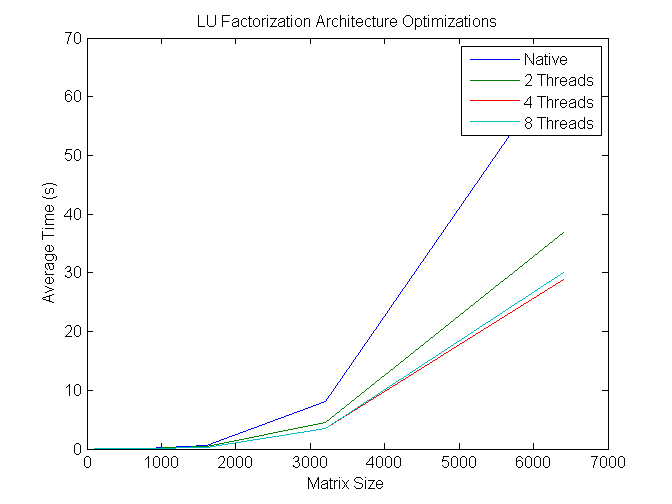
\includegraphics[scale=0.5]{figures/fig5}
\end{center}

\end{frame}

\begin{frame}
\frametitle{Conclusion}
\begin{itemize}
\item Free 4.75x speedup with just compiler flags
\item 10 x speedup by targeting multi-core machines
\item Don't need to sacrifice code readability for performance
\item Vectorization didn't help as much as expected
\end{itemize}
\end{frame}



\end{document}